%   Drones
%
%   Fall 2015
%
%  last modified 11/4/2015,   sy457
%

\documentclass{article}
\usepackage{epstopdf}
\usepackage{graphics}
\usepackage{graphicx}
\usepackage{amsmath}

\usepackage{tikz}
\usepackage{pgfplots}
\usepackage{listings}
\usepackage{csvsimple}
\usepackage{nicefrac}
\usepackage{units}
\usepackage{subfig}
\usepackage{breqn}

\linespread{1.6}

\title{Project II: Big Brother is Watching You!}
\date{2015-11-02}
\author{Albert Quizon, Christopher Silvia, Siyu Yang}
\begin{document}

\maketitle

\begin{abstract}
   abstract-text
\end{abstract}

\newpage

\section{Instructions}
The problem requires us to develop a MAV surveillance scheme across a hypothetical area -- Gotham City, with the goal to completely patrol the given area. The scheme are subject to the four following constraints:
\begin{itemize}
\item Every given geographic point in the city needs to be covered on 15 minutes periods
\item The flight plan needs to miniminze sharp turns, take into consideration refueling stops, and a possible scheme of 30% contingencies
\item The flight plan needs to cover the area around Gotham University and Financial Districts on 5 minutes periods, and Gotham Central Park once in 20 minutes
\item The flight plan needs to be randomized for the sake of fairness against "insider jaywalking"
\end{itemize}
All four constraints need not to be satisfied at the same time.

\section{Model Assumptions}
\section{Parameter Values and their Justifications}
\subsection {Gotham City}
As the original construction in the Batman Series, Gotham City is New York City Mahattan area below 14th Street. For simplicity, we are assuming that Gotham City is a 3 miles – by – 3 miles square area. Gotham University (a fictional depiction of NYU), the Financial District and Gotham Central Park are reduced respectively to a $0.5 \times 0.5$,  $1 \times 1$ square miles square areas and a $1 \times 1$ square miles square areas. Assume the two areas are seperate.
\subsection{Technical Data for UAV}
The work \textit{Drones And Aerial Observation} introduced an equation regarding Ground Sampling Distance (GSD) – the area a drone will be able to observe at a given cruise height:
\begin{equation}
GSD = \frac{\text{pixel size x height above ground level}}{\text{focal length}}
\end{equation}
If we assume that the drone is armed with Canon S100, a most common filming device used by UAVs, we will have a camera with pixel size of 0.0019mm, focal length ranging from 24 – 120mm, and can produce images of up to 4,000 by 4,000 pixels. Assuming a cruise height of 1000 meters, we will be able to get a 1000 ft by 1000 ft surveillance vision every given moment.

From \textit{Drones And Aerial Observation}, we know that for common UAV used in mapping and survellance, it is reasonable to consider its flight speed as 16 meters per second.
\subsection{Assumptions for drone behaviors}
We will make the following 
\begin{itemize}
\item Drones can start anywhere and can come down for recharging/refueling at any point on the grid. 
\end{itemize}
\section {Simulation Algorithm}

\subsection{Model I: Rectangular Patrol Path}

For the first simple discrete model, we are going to estimate where every single drone would cover a given square area on the map. For any given drone, it will be patrolling a given rectangular area. We need to make sure in the interval of 15 minutes (900 seconds), the drone will cover the whole area. Thus we are considering a 304.8 meter (1000 feet) wide "snake" drawing out a rectangular region for all 15 minutes, with ground speed 16 meters per second (35.71 miles per hour). The path covered would be individualized for each drone, as in Figure \ref{M1Path1}. This would cover:

\begin{figure}[htb!]
\begin{center}
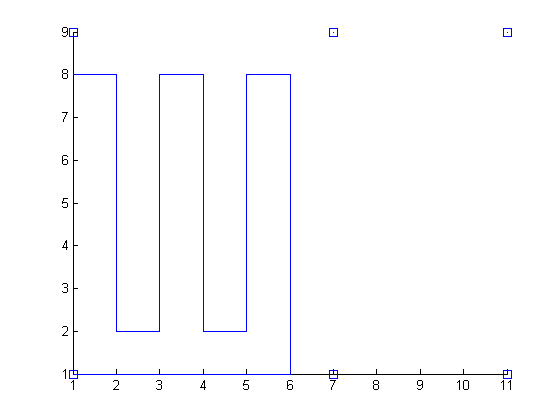
\includegraphics[width=3.2in]{M1Path1.png}
\end{center}
\caption{Path of one drone after one cycle of 15 minutes.
\label{M1Path1}}
\end{figure}

\begin{equation}
35.71 \unitfrac{mi}{hr} \times 15 minute \times 1000 feet = 1.7 miles^2
\end{equation}

To cover all of Gotham City (assumed as a 4828 by 4828 meters$^{2}$ square = 23,309,584 $[m^{2}]$) in 15 minutes, we need at least 6 drones ($\frac{23309584}{4389120} = 5.31$). 

We can see that the above model is very crude and limited. It assumes that the drones would draw out 4,389,120 $[m^{2}]$ rectangles on the map for 15 minutes (without considering refueling). 

In order to create a model for this discrete method, we had to assume a square map of Gotham, where a drone can observe a square area of 304.8 meters by 304.8 meters. We had to break down the Gotham area into a discrete set of grid points, where the spacing between each point was twice the radius of observation of a drone (304.8 meters). After doing some calculations shown in the code provided in Appendix Listing 2, we determined we needed 256 "blocks" to cover all of Gotham. Each drone could cover 48 of those blocks in a 15 minute interval. We used two arrays. One array was designed to keep track of the current location of each drone and another array was designed to keep track of time since that area was last observed. We do have to make the assumption that the drones can start anywhere and can come down for recharging/refueling at any point on the grid. We implemented a check to see if any block in the array was not observed in a 15 minute interval. A visual of the paths and positions the drones took are provided in Figure \ref{M1Path}.

\begin{figure}[htb!]
\begin{center}
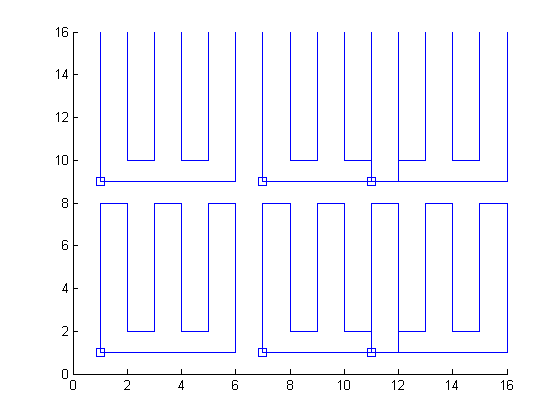
\includegraphics[width=3.2in]{M1Path.png}
\end{center}
\caption{Path of 6 drones after one cycle of 15 minutes.
\label{M1Path}}
\end{figure} 

The blue squares represent the location of each drone at a given time, and the blue lines are the path that each drone took. There were no failures to observe any point in the grid after running the code for multiple cycles. There were some overlaps in the paths of some drones, so some areas of the map were observed more frequently than once every 15 minutes but the figure verifies that we need at least 6 drones watching the city at all times.

The better alternative to this form of solution is to create a large U-based path that traverses the whole array. This allows for even spacing between the drones, so all the areas of the map will be observed at the same frequency. While this method provides a better distribution of observation time to each point, it also safeguards against any failures in drones. If a percentage of the drones fail, then we will still maintain coverage of the whole area of Gotham without having to reprogram any drones or send new ones. The drones would take on a path similar to the one shown in Figure \ref{Comb}.  

\begin{figure}[htb!]
\begin{center}
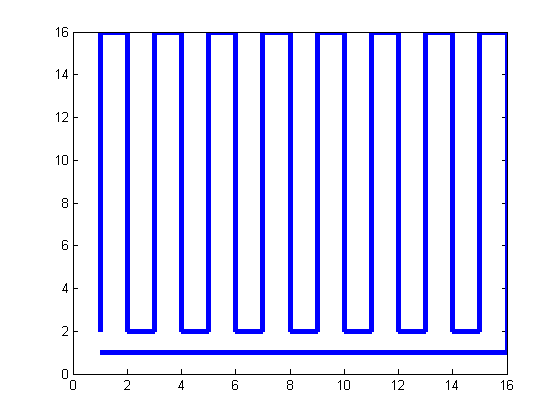
\includegraphics[width=3.2in]{Comb.png}
\end{center}
\caption{Path of 6 drones in a large comb pattern.
\label{Comb}}
\end{figure}


\newpage 
\subsection{Strategy II: Variable Levels of Coverage}

In order to increase patroling around Gotham University and Financial district to every 5 minutes, and the rest of the area every 20 minutes, we have the designated patrol area of every drone around critical region, we implete a discrete strategy similar to the one offered above. In this case, to increase the patrol period means to decrease the area patroled:
\begin{equation}
35.71 \unitfrac{mi}{hr} \times 5 minute \times 1000 feet = 0.6 miles^2
\end{equation}
and patrol area of every drone around none-critical region:
\begin{equation}
35.71 \unitfrac{mi}{hr} \times 20 minute \times 1000 feet = 2.5 miles^2
\end{equation}

With simple math we can find that this means we need 1 drone to continuously patrol the $0.25$ square miles of region around Gotham University, and 2 drones to patrol the area around Financial district. For the rest of area including Gotham Central Park, we would need 3 other drones to cover. We can easily implement the need for refueling every 5 hours by providing another set of 6 drones which will take over for the first set of drones while they recharge. We make the assumption that drones can recharge/refuel in under 5 hours. This means the city needs at least 12 drones to monitor that no point in the city goes unobserved for more than 15 minutes in a row. 

We can see that the above model is also very limited. It assumes that the drones would draw out $9 miles \times 1000 feet $ rectangles on the map for 15 minutes, without considering refueling, turns and cost. Areas around Gotham University and Financial districts are over patrolled, resulting in higher cost. Moreover, the patrol routes are fixed, resulting in no randomness and thus could easily calculate a jaywalk route without getting caught. 

\newpage

\subsection{Strategy III: Contingencies}

This model involves the usage of fuel with respect to the motion of the drone. Paths requiring more sharp turns will require more frequent recharging/refueling stops. We will also have to consider that the MAVs are not very reliable so a significant proportion of them might be briefly grounded for repairs. However, we have to implement a plan to ensure that even if some drones go down, all areas of the city will be observed even if somewhat less often. We make the assumption that 30 \% of the drones will become unusable. 

The first problem to address is the use of fuel. More turns means more fuel consumed, so the number of terms is our constraint. We can still assume that each drone can observe their own area, so we have to apply a minimization of the number of turns for the path of each drone. We can also assume that the areas still have to be observed at least once every 15 minutes. There are a few conditions regarding the path of each drone:

1. The path of the drone must touch each node of its respective grid. 

2. The path of the drone cannot self-intersect.

3. The path of the drone must return to start at the end of 15 minutes. 

We must satisfy all of these conditions. There are only two general paths we can draw to fulfill these conditions. The first is an H-like path, as shown in Figure \ref{Paths}a. The second is a U-like path, as shown in Figure \ref{Paths}b. The H path needs 11 turns to complete the path while the U path only needs 7 turns. Therefore, the most fuel efficient path is the U path. 

There is another problem of having the drones refuel at least every 5 hours. The optimal number of drones in this case would be based on the amount of time needed for refueling, which we assume to be less than the length of time it can fly for. Based on this assumption, we have a formula to determine how many drones we need. O is original number of drones needed, N is number of backup drones needed (drone stations where we can recharge), L is length of duration of flight for each drone, R is time needed to refuel. The first assumption we need in this case is to stagger when we put each drone up in the air. The maximum time we can stagger each drone by is:

\begin{eqnarray*}
T_{stagger} &=& \frac{L}{O}N	\\
\end{eqnarray*}

This is dependent on how many backup drones we have  (which we can treat as drone stations to simplify things). Therefore, each drone that comes into each station will be empty on fuel and will need to completely refuel. Our constraint then is that the time interval has to be greater than the refueling time. 

\begin{eqnarray*}
\frac{L}{O}N &\geq & R	\\
N &\geq & \frac{(R)(O)}{T}	\\
\end{eqnarray*}

As a result, Number of drones $\geq$ $\frac{(Time~needed~to~refuel)(Original~Number~of~Drones)}{(Length~of~duration~of~flight)}$. 

We have O = 6 drones, and L = 5 hours, but now we can solve for number of drones given the time needed to refuel. If the drones need 5 hours to completely refuel, then we would need 12 drones. 

The next problem is to consider contingency plans for when some drones become unusable. 

\begin{figure}%
    \centering
    \subfloat[H Path of a drone given even number of grid squares]{{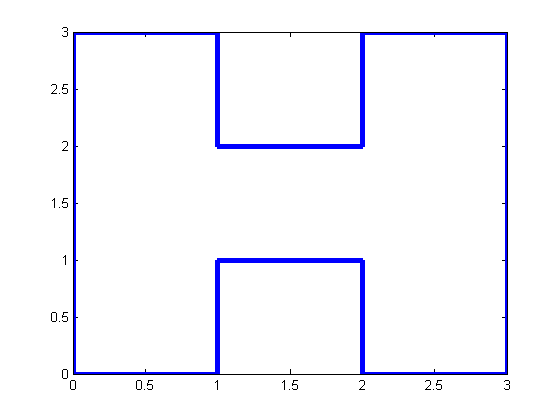
\includegraphics[width=4cm]{HPath.png} }}%
    \qquad
    \subfloat[U Path of a drone given even number of grid squares]{{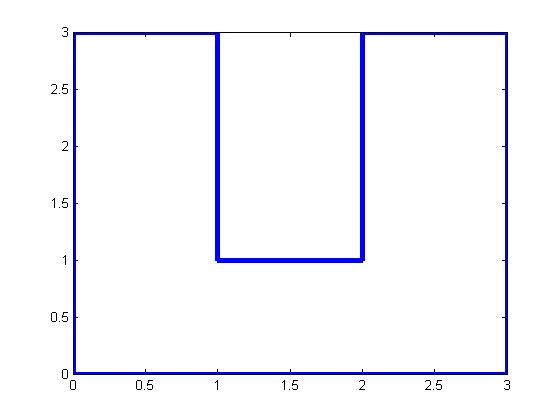
\includegraphics[width=4cm]{UPath.png} }}%
    \caption{H and U Paths of a drone}%
    \label{Paths}%
\end{figure} 

If 30 \% of the drones become unusable, then the simplest way of addressing the issue is to just replace them by having 30 \% more drones to replace the ones that break. We will need at least 12 drones to patrol every point at least once every 15 minutes. From this, we know we will need a total of 18 drones, where 30 \% of these (5.4) will become unusable. When any drone fails, we can just send another up in its place. There is also the option of reprogramming the drones to assume new paths. This is the most basic strategy to this problem. 

However, our goal should be to implement a strategy which covers all of the area even if 30 \% of the drones go down. Ideally, we should not have to reprogram the drones or send more in from storage. The way to do this is by creating a large cycle which should minimize the number of turns and fuel. We already proved earlier that the best shape for the paths in a given area are U shaped, so we can implement a "comb" like path to traverse the whole map, like in Figure \ref{Comb2}. 

\begin{figure}[htb!]
\begin{center}
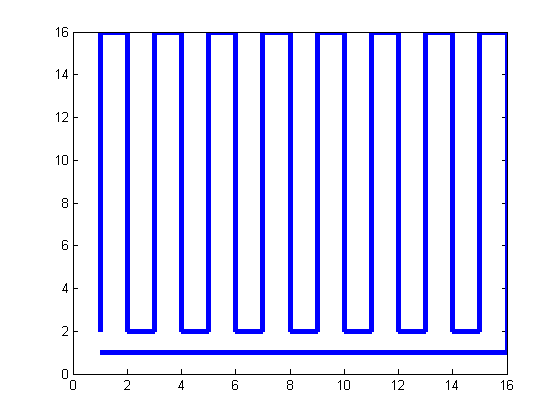
\includegraphics[width=3.2in]{Comb.png}
\end{center}
\caption{Path of 6 drones in a large comb pattern.
\label{Comb2}}
\end{figure} 

To go further with this model, we can actually create a comb like pattern for the entire grid and use the drones to traverse the comb pattern to accomplish surveillance. We will still have 256 grid points to observe, but if we evenly distribute the 6 drones along the path, we can then have them observe 43 (256/6, rounded up) spaces each before the next drone retraces those same spaces. The time it takes to traverse a path of 43 tiles is 806.25 seconds, or 13.44 minutes. From this, we can determine that each area in Gotham city under this method will be observed at least once every 13.44 minutes, which is even better than the desired 15 minutes. 

Now we have to account for the 30 \% rate that the drones will fail. That means that of the current 6 that we have running, about 2 of them will fail. We will then have a total of 256 tiles to cover between 4 drones. 

The best case would be if the two drones were not consecutive and only left gaps of 86 tiles. This means that any point in the map could go unobserved for 1612.5 seconds, or 26.875 minutes. 

In the worst case, the 2 drones that become unusable are consecutive drones along the path. Since the drones were split apart by 43 tiles, then we will be left with an 129 tile gap. This means that any point in the map can go unobserved for a maximum of 2418.75 seconds or 40.3125 minutes. 

Given a strategy to assume a "comb" like path and a 30 \% failure rate of drones, the maximum any point in the map can go unobserved for is 40.3125 minutes and the minimum is 27.875 minutes. 


\subsection{Strategy IV: Ideal Gas Model}

\subsubsection{Problem Statement}

\paragraph{}
For the final scenario, we need to program the drone paths so that our insider
	knowledge about the drones' plans cannot be used to give us (the modelers)
	the ability to plan an observation-free jaywalking path through Gotham.
This severly limits the amount of structure our model can have.
Our model cannot have a fixed schedule for drone movements;
	we (the modelers) would then be able to avoid the drones.
We could have random drones scheduled on fixed routes, but our knowledge of the
	routes would allow us (the modelers) to go to low-observability regions,
	and perhaps use spotters to determine when drones were dispatched on routes.

\subsubsection{Description of Model}

We have therefore chosen not to use fixed routes for this model.
Instead, the drones will travel in straight lines at fixed velocities within 
	the borders of Gotham, and bounce off of the boundaries when they reach them  
	(See Figure \ref{fig:drone-barrier-bounce}).
If the drones occasionally change their directions randomly, then they should
	be uniformly distributed throughout Gotham.
If the drones are uniformly distributed throughout Gotham, then the modelers
	will not be able to plan low-observability paths, since each part
	of Gotham has the same chance of being observed as any other.

\begin{figure}[h]
\begin{center}
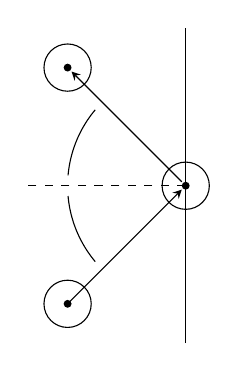
\begin{tikzpicture}

% wall/boundary for drone to bounce off of
\draw (1,-2) to (1,2);

% drone before bounce
\draw (-0.5,-1.5) circle (0.3);
\fill (-0.5,-1.5) circle [radius=0.05];

% drone during bounce
\draw (1.0, 0.0) circle (0.3);
\fill (1.0, 0.0) circle [radius=0.05];

% drone after bounce
\draw (-0.5, 1.5) circle (0.3);
\fill (-0.5, 1.5) circle (0.05);

% bouncing arrows
\draw[->,>=stealth] (-0.5, -1.5) -- (0.95,-0.05);
\draw[->,>=stealth] (0.95, 0.05) -- (-0.45, 1.45);

% line of symmetry
\draw[dashed] (1,0) to (-1,0);

% angle measures
\draw[domain=140:175] plot ({1 + 1.5*cos(\x)}, {1.5*sin(\x)});
\draw[domain=-175:-140] plot ({1 + 1.5*cos(\x)}, {1.5*sin(\x)});

\end{tikzpicture}
\end{center}
\caption{An incoming drone bounces off of a barrier.  The circle is its radius
	of vision.
Note that if the wall extends in the $y$ direction, the bouncing just 
	multiplies the $x$ component of the velocity by $-1$.}
\label{fig:drone-barrier-bounce}
\end{figure}


Suppose there is a domain with area $A$, which contains a single drone.
The drone moves at a constant velocity $v$, and observes a radius $r$ around it.
The direction of the drone, and its position, are both uniformly random at time $t=0$.
Consider a target point, $x_t$, within $A$.
We are interested in how likely the drone is to intersect the point $x_t$ in a
	given time interval.
This situation is shown in Figure \ref{fig:drone-in-random}.

\begin{figure}[h!]
\begin{center}
\begin{tikzpicture}

\coordinate (x-t) at (0.2, 1.4);
\node[right] (x-t-label) at (x-t) {$x_t$};
\fill (x-t) circle (0.05);

\coordinate (drone-position) at (0.0,0.0);
\fill (drone-position) circle (0.05); 
\draw (drone-position) circle (0.3);

\draw[->] (drone-position) to (0.9,0.6) node[below] (arrow-endpoint) {$v$};
\draw plot [smooth cycle] coordinates {(0,-1.5) (2.5,-0.5) (1.5,2.0) (2.0, 3.0) (0.0, 3.5) (-1.5,1.5)};

\end{tikzpicture}
\end{center}
\label{fig:drone-in-random}
\caption{A drone moves through $A$ with constant velocity $v$}
\end{figure}

\subsubsection{Analytical Formula for Observation CDF}

We are interested in determining whether the target is observed between times $0$ and $t$.
Since the drone is uniformly distributed throughout the domain $A$, as long as it is
	not near the boundary of $A$, the drone should fly in a straight path covering a distance
	$v t$, and observe the area shown below:

\begin{figure}[h!]
\begin{center}
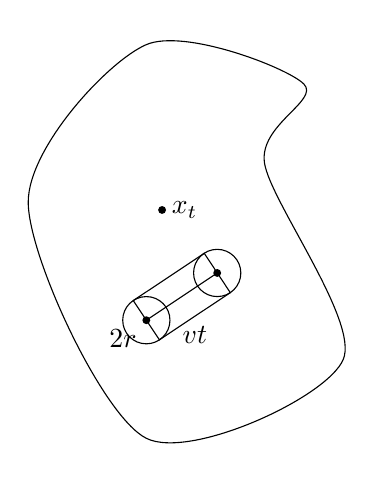
\begin{tikzpicture}

\coordinate (x-t) at (0.2, 1.4);
\node[right] (x-t-label) at (x-t) {$x_t$};
\fill (x-t) circle (0.05);

\coordinate (drone-initial-position) at (0.0,0.0);
\fill (drone-initial-position) circle (0.05); 
\draw (drone-initial-position) circle (0.3);

\coordinate (drone-final-position) at (0.9,0.6);
\fill (drone-final-position) circle (0.05); 
\draw (drone-final-position) circle (0.3);

\draw (drone-initial-position) to (drone-final-position);
\draw plot [smooth cycle] coordinates {(0,-1.5) (2.5,-0.5) (1.5,2.0) (2.0, 3.0) (0.0, 3.5) (-1.5,1.5)};

\coordinate (top-left-corner) at (-0.166, 0.2496);
\coordinate (bottom-left-corner) at (0.166, -0.2496);
\coordinate (top-right-corner) at (0.7359, 0.8496);
\coordinate (bottom-right-corner) at (1.0664, 0.350);

\draw (top-left-corner) 
	to node[below left] (2r) {$2 r$} (bottom-left-corner) 
	to node[below] (vt) {$v t$} (bottom-right-corner) 
	to (top-right-corner) 
	to (top-left-corner);

\end{tikzpicture}
\end{center}
\label{fig:drone-coverage-area}
\caption{In time $t$, the drone covers area $\pi r^2 + 2 r (v t)$}
\end{figure}

Since the drone's position and velocity are uniformly randomly distributed,
	the shape in Figure \ref{fig:drone-coverage-area} is approximately equally likely to 
	cover any point in $A$.	
Approximation errors come from the boundaries of the region: if the drone bounces
	off the boundary between $t=0$ and $t=t$, then the area covered is not
	$\pi r^2 + 2 r (v t)$.
If there is significantly more area than boundary, however, than the chance of being 
	observed between $t=0$ and $t=t$ is just the fraction of $A$ which is observed,
	which is:

\begin{align}
P(t) & = \frac{\pi r^2 + 2 r (v t)}{A}
\end{align}

\begin{figure}[h!]
\begin{centering}
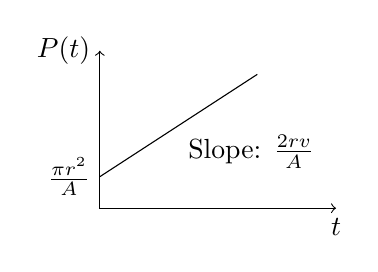
\begin{tikzpicture}

\draw[<->] (0,2) node[left] (yaxis) {$P(t)$} |- (3,0) node[below] (xaxis) {$t$};

\coordinate (yintercept) at (0,0.4);
\node[left] (p-of-zero) at (yintercept) {$\frac{\pi r^2}A$};
\draw (yintercept) to node[below right] (middle) {Slope: $\frac{2 r v}{A}$} (2.0, 1.7);

\end{tikzpicture}
\label{fig:p-plot}
\caption{Plot of the Cumulative Probability of being observed by a single drone,
between times $0$ and $t$.
Note that this model breaks down at or before $t = \frac{ A - \pi r^2 }{2 r v}$,
	when the model predicts $P(t) = 1$.}
\end{centering}
\end{figure}

\subsubsection{Multiple Drones}

If there are multiple drones, and the probability of being observed by one of them between
	$t=0$ and $t=t_f$ is $P(t)$, then the probability of being observed by any one of them
	is equal to the probability of \emph{not} being observed by \emph{none} of them:

\begin{tabular}{r|l}
Between $t = 0$ and $t = t_f$, for $t_f$ small & Probability \\
\hline
Observation from a single drone. & $P(t)$\\
No Observation from a single drone. & $1 - P(t)$ \\
No Observation from $n$ independant drones & $\left(1 - P(t)\right)^n$\\
At least one Observation from $n$ independant drones 
	& $1 - \left( 1 - P(t) \right)^n$\\
\end{tabular}

Therefore, when $t << \frac{A - \pi r^2}{2 r v}$, the probability
	of being observed by at least one drone in the interval from $0$ to $t$
	is given by:

\begin{align}
P_n(t) & = 1 - \left( 1 - \frac{\pi r^2 + 2 r (v t)}{A}\right)^n
\end{align}

Notice that for any $\lambda$, $P_n(t)$ is unchanged if the parameters
	$r$, $v$, and $A$ are rescaled as follows:

\begin{align*}
	r & \to \lambda r\\
	v & \to \lambda v\\
	A & \to \lambda^2 A 
\end{align*}

To see this, we can apply this rescaling to $P_n(t)$:

\begin{align*}
1 - \left( 1 - \frac{\pi r^2 + 2 r (v t)}{A}\right)^n
	& \to 1 - \left( 1 - \frac{\pi (\lambda r)^2 + 2 (\lambda r) ((\lambda v) t)}A
		\right)^n\\
	& \to 1 - \left( 1 - \frac{\lambda^2}{\lambda^2} \frac{\pi r^2 + 2 r (v t)}A
		\right)^n\\
P_n(t) & \to P_n(t)
\end{align*}

Therefore, $P_n(t)$ is independant of the ``length-scale'' of the problem.
If we express time in units of $\frac1v$, then the value of $v$ becomes 
	unimportant.
We can chose $\lambda = +\frac1{\sqrt{A}}$, so that the rescaled $A$ is 
	1.
Therefore, the only relevant quantity is the normalized radius of the drone,
	which is best expressed by the ratio $\frac rA$.


\begin{figure}[h!]
\begin{centering}
\pgfplotstableread[col sep = comma]{pn-curves.csv}\mydata
\begin{tikzpicture}
	\begin{axis}[
		xmin = 0,
		xmax = 15,
		ymin = 0,
		ymax = 1,
		xlabel = {$t$, units of $\frac1v$},
		ylabel = {$P(t)$}]
	\foreach \index in {1,...,20} {%
		\addplot[mark=''] table[x index = 0, y index = {\index}]{\mydata};
	}
	\end{axis}
\end{tikzpicture}
\label{fig:p-curves}
\caption{Expected values for $P(t)$. Here $A = 6.0, r = 0.1$, $\frac rA = 0.0166$.}
\end{centering}
\end{figure}

\subsubsection{Validating the Expected Number of Drones}

We implemented a model which simulates the movement of drones within a $3$ by $2$
	rectangle.
The drones bounce off of the walls as described.
We recorded the amount of time spent $t$ or fewer minutes from the next
	observation, and by dividing by the total simulation time,
	converted that into an expected probability of observation within the
	next $t$ minutes.

The model's predictions hewed to our predictions uncannily well.
They are presented below:

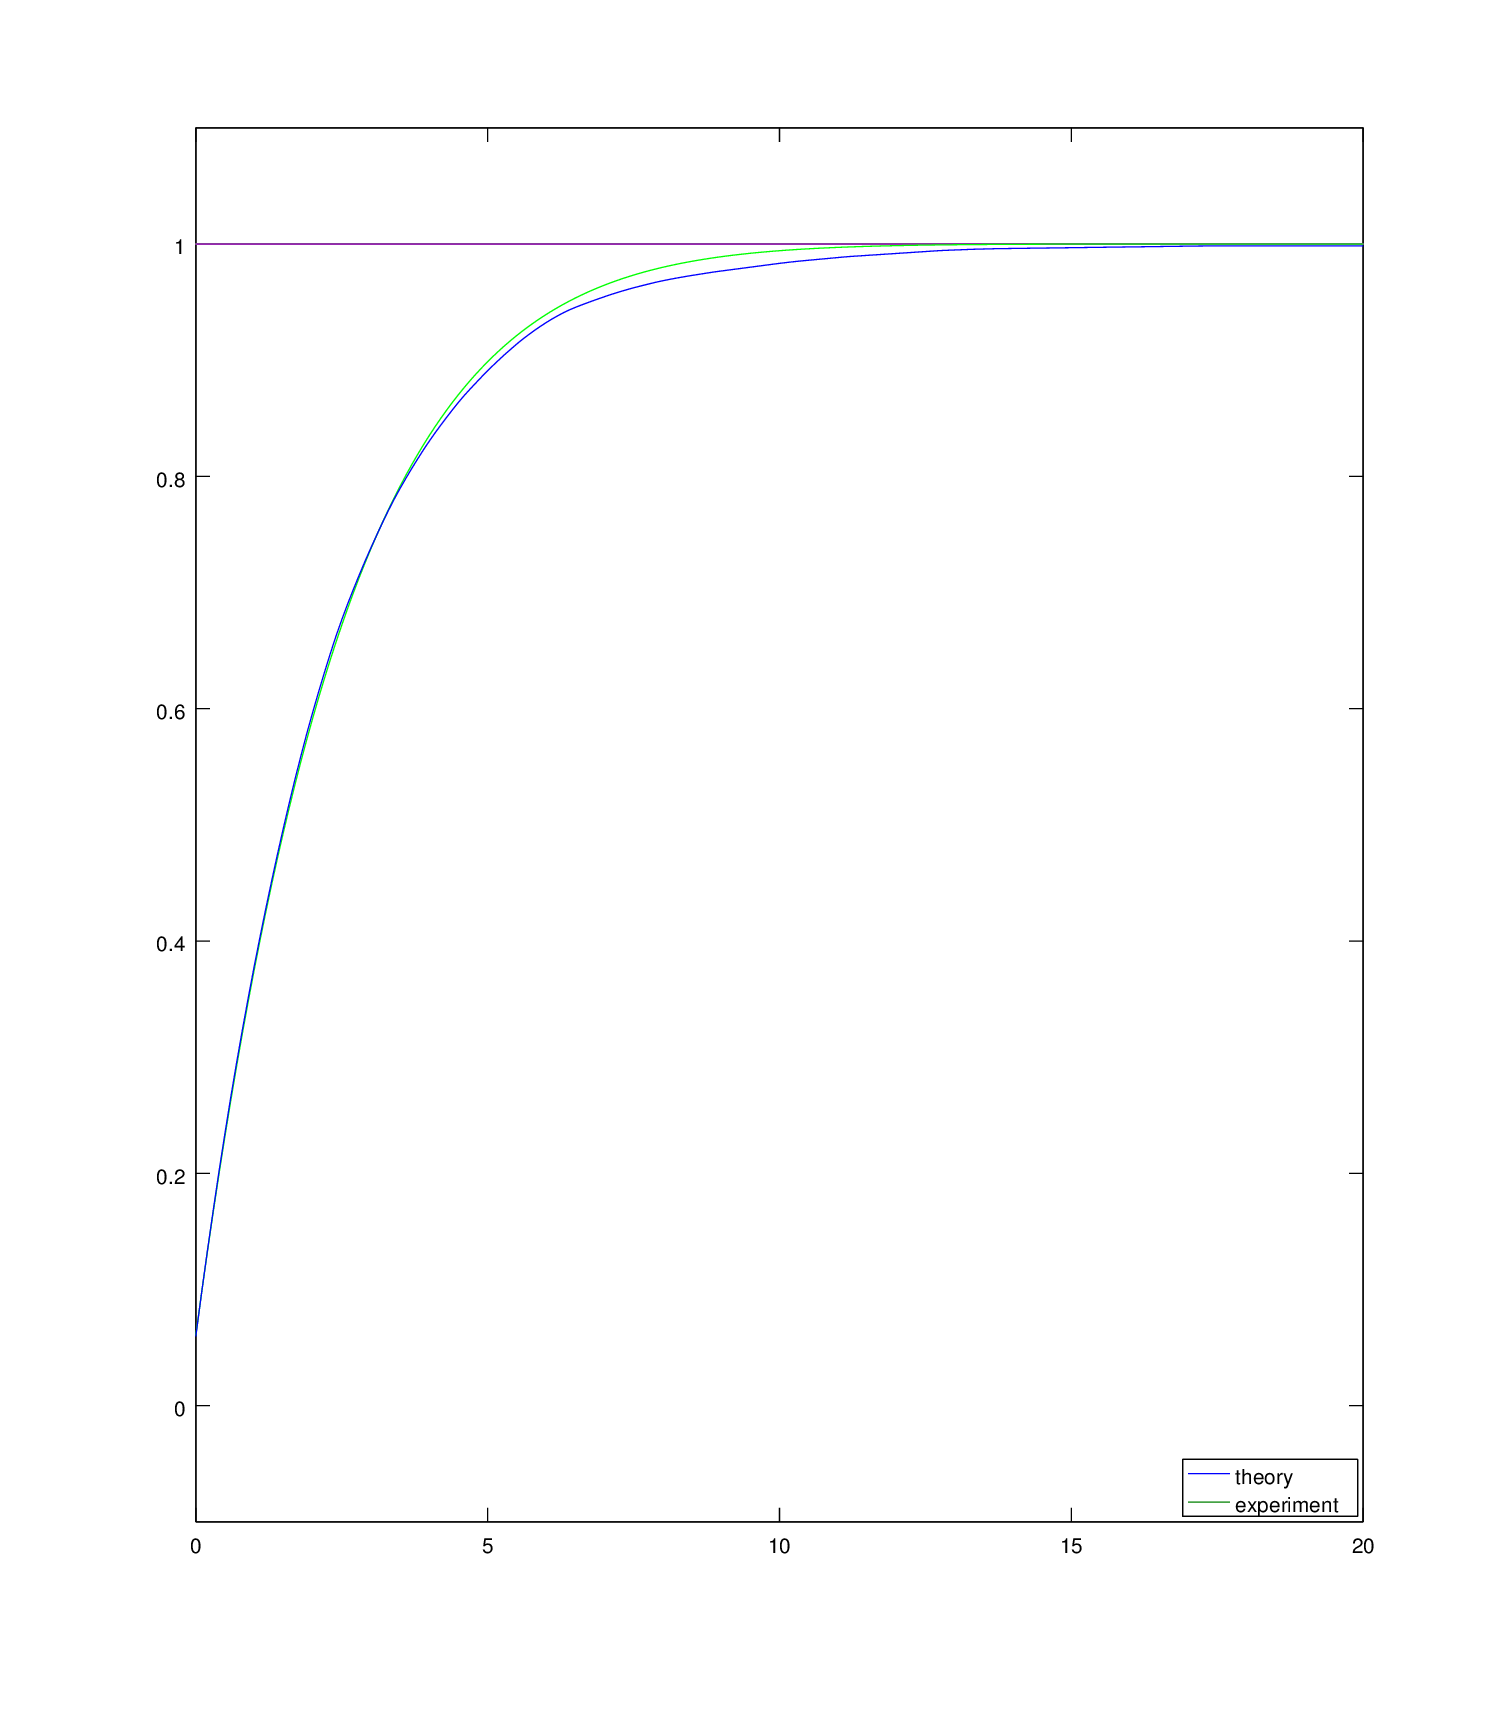
\includegraphics[width=\textwidth]{theory-vs-experiment.png}

Our model underestimates the probability, but only by a very small amount.
The code for this images is presented in the code appendix.

\subsubsection{How Many Drones to Buy?}

Suppose the goal of a drone purchasing program is:
	achieve $f(t)$-percent coverage after $t$ time units.
With $n$ drones, the chance of being observed after $t$ time units is:

\begin{align}
f(t) & = 1 - \left( 1 - \frac{\pi r^2 + 2 r (v t)}{A} \right)^n
\end{align}

Therefore, solving for $n$:

\begin{align}
n & = \frac{\log\left(1 - f(t)\right)}{\log\left( 1 - \frac{\pi r^2 + 2 r (v t)}{A}\right)}
\end{align}

Earlier we determined the following parameter values:

\paragraph{}
\begin{tabular}{l|l}
Parameter & Value \\
\hline
A & $(4.828 $km$)^2$ or $23,309,584 m^2$ \\
r & $300 m$ \\
v & $16 m/sec$
\end{tabular}
\paragraph{}

If we want to be observed every 15 minutes $95 \%$ of the time, 
	this will require 6.2081 drones.
We can round up to 7 drones.

\subsubsection{Robustness Testing}

Suppose $v$ is smaller than it should be.
This could happen for many reasons: there could be rain which impedes
	the motion of the drones, there could be a power shortage, there
	could be interfering regulations.
We want to see how this change in $v$ will affect our predictions.

\begin{figure}[h!]
\begin{centering}
\pgfplotstableread[col sep = comma]{robustness.csv}\otherdata
\begin{tikzpicture}
	\begin{axis}[
		xmin = 0,
		xmax = 30,
		ymin = 0,
		ymax = 1,
		xlabel = {$v$, $m/sec$},
		ylabel = {$P(t =$ 15 minutes$)$ from new $v$}]
	\addplot[mark=''] table[x index = 0, y index = 1]{\otherdata};
	\addplot[mark=''] coordinates { (16.0, 0.0)
							(16.0,1.0) };
	\addplot[mark=''] coordinates { (0.0, 0.95)
							(30.0, 0.95)};
	\end{axis}
\end{tikzpicture}
\caption{Robustness Test for Changed Velocity Values.
If the velocity is above about $15 m/sec$, then the desired 95\%
	coverage is still achieved.}
\label{fig:robust}
\end{centering}
\end{figure}

In Figure \ref{fig:robust}, we show how the probability of having been
	observed after 15 minutes decays as the velocity decreases.
The rounding-up to have an integral number of drones has helped, and the
	velocity can dip down to $15 m/sec$ without disruptions.

\subsubsection{Model Conclusion}

This model shows that random observations are competitive with hand-engineered
	models, since it only calls for seven drones.
The model shows that the velocity of the drones is a vital parameter,
	since the amount of observations decay rapidly with the velocity, 
	as is the radius of observation.
The model's expected values agree very well with computational experiments,
	so they can be trusted.
In conclusion, this model accurately predicts how many drones to buy to achieve
	a desired level of coverage.

\subsubsection{Further Work}

Some further things we could do:
We could instruct the drones to maneuver in order to avoid each other,
	to avoid overlapping.
We could also work on ways of making the drones avoid each other,
	or move towards points which have not been observed for a long time.

\section{References}

%	\section{Math Appendix}
%	
%	In the fourth model, we mentioned that there was a rigerous mathematical
%		derivation of the $\frac{\pi r^2 + 2 r (v t)}{A}$ rule.
%	We present it below:
%	
%	We desire to find the probability that a point $x_c$ is observed between
%		times $0$ and $t$.
%	We assume that the drone is uniformly distributed throughout the domain,
%		and that the boundary of $A$ is further from $x_c$ than $vt + r$,
%		the largest distance away from $x_c$ that a drone can start and still
%		observe it by time $t$.
%	We further assume that the drone velocity direction is uniformly distributed
%		as well.
%	
%	First, we will find the probability that a drone a distance $a$ away from	
%		$x_c$ is on a trajectory to observe $x_c$ within $t$ seconds.
%	If $a < r$, then the drone is already observing $x_c$, so the probability
%		is 1.
%	
%	\begin{figure}[h!]
%	\begin{tikzpicture}
%	\coordinate (xc) at (0.0, 0.0);
%	\node[left] (xclabel) at (xc) {$x_c$};
%	\fill (xc) circle (0.05);
%	
%	\coordinate (drone) at (4.0, 0.0);
%	\draw (xc) to node[above] {$a$} (drone);
%	\fill (drone) circle (0.05);
%	\draw (drone) circle (0.5);
%	
%	\coordinate (just-miss) at (0.0, -0.5);
%	\draw (xc) to node[left] {$r$} (just-miss);
%	
%	\draw (just-miss) to node[below right] {$d < v t$} (drone);
%	\fill (just-miss) circle (0.05);
%	\draw (just-miss) circle (0.5);
%	
%	\end{tikzpicture}
%	\caption{If the drone is closer than $\sqrt{(vt)^2 - r^2}$, 
%		then the drone will always make it in time.
%	It only matters if it misses or not}
%	\end{figure}

\section{Code Appendix}
\lstinputlisting[language=octave,
	caption={Ideal Gas Simulation}, 
	label=code:ideal-gas]
{gas-expectation-validation.m}

\lstinputlisting[language=Matlab,
	caption={Basic Coverage}, 
	label=code:Basic]
{Strategy1.m}


\end{document}
